\chapter{Evaluation}

\todo[inline]{Im vorhergegangenen Kapitel wurde beschrieben, [wie die Netze designed wurde]
Jetzt bewerten wie gut sie das eigentlich mache.}

\section{System}

Alle in dieser Arbeit vorgestellten Netze wurden auf einem Ubuntu 18.04 Linux System trainiert und evaluiert.
Dieses verfügte über einen Intel i7-7700k CPU @ \SI{4.20}{\giga\hertz}, eine NVIDIA GeForce 1080Ti Grafikkarte mit \SI{11}{\giga\byte}~GDDR5X,
und \SI{32}{\giga\byte}~RAM. 

\todo[inline]{muss da noch irgendwie mehr dazu?}

\section{Vergleichsmodelle}

\color{blue}
Notation und Definition bei allen diesen Modellen nach Florian's Diss \cite{Pfaff2018}, mit Ausnahme von Average Acceleration.
Sei \(x(t)\) die Position des Partikels entlang der Bewegungsrichtung in Abhängigkeit von der Zeit
(continuous-time equation).
Sei \( y(t)\) die Position des Partikels orthogonal zur Bewegungsrichtung in Abhängigkeit von der Zeit.
\(t^{\text{Last}}\) ist der Zeitpunkt der Beobachtung des letzten Features.
% Sei \(\Delta t =  t - t^{\text{Last}}\).

Vergleich über Boxplots: Balken: 25\%-Quantil bis 75\%-Quantil.
Roter Balken ist der Median. Der obere und der untere Whisker 
gehen bis zum höchsten bzw. niedrigsten Wert, der nicht mehr als 2.7 Standardabweichungen vom Median abweicht
Die Outlier werden nicht angezeigt.

\color{black}

In diesem Abschnitt sollen die Modelle eingeführt werden, mit denen die Ergebnisse der Neuronalen Netze verglichen werden.
Mit Ausnahme des \textit{Average Acceleration} Modells stammen sie alle aus \cite{Pfaff2018} und sowohl Definition als auch Notation wurden von dort übernommen.
Dabei seien \(x\) die Achse entlang der Bewegungsrichtung des Förderbands und \(y\) die Achse orthogonal zur Bewegungsrichtung des Förderbands.
Zeitdiskreten Messungen entlang der einzelnen Achsen werden als \(\mathsf{x}_t\) beziehungsweise \(\mathsf{y}_t\) dargestellt.
Die daraus rekonstruierten zeitkontinuierlichen Positionsgleichungen als \(\mathsf{x}(t)\) beziehungsweise \(\mathsf{y}(t)\).
Sei \(t^{\text{Last}}\) der Zeitpunkt der Beobachtung des aktuellsten Features und \(x^{\text{Last}}\) und \(y^{\text{Last}}\) die dazugehörigen Positionen entlang der beiden Achsen.
Sei \(\mathsf{x}^{\text{PredTo}}\) die Position des Druckluftdüsenarrays entlang der \(x\)-Achse.
Sei \(t^{\text{Pred}}\) der Zeitpunkt an dem ein Partikel den Druckluftdüsenarray passiert.
Sei \(\mathsf{y}^{\text{Pred}} = \mathsf{y}(t^{\text{Pred}})\) die Position entlang der \(y\)-Achse an dem der Partikel den Druckluftdüsenarray passiert.
\(\Delta t = t^{\text{Pred}} - t^{\text{Last}} \) und \(\mathsf{y}^{\text{Pred}}\) dementsprechen den Labels der einzelnen Feature-Label-Paare für das Separator Netz.
\(\mathsf{x}(t^{\text{Last}} + 1)\) und \(\mathsf{y}(t^{\text{Last}} + 1)\) entsprechen den Labels der Feature-Label-Paare für das NextStep-Netz.
Die verschiedenen Modelle können nun ebenso wie die Ergebnisse der verschiedenen Netze bewertet werden, 
indem man die Abweichung zwischen dem Ergebnis in dem Modell und der Ground Truth in den Feature-Label-Paaren bestimmt.
\todo{Das formatting hier ist total schlecht - überlegen wie ich das gut machen kann.}


Für Modelle, die unabhängig von der Beschleunigung der Teilchen sind, ist der Zustandsvektor wie folgt definiert:

\begin{equation} \label{eq:definitionCV}
    \vx(t) = 
    \begin{bmatrix}
        \mathsf{x}(t) \\
        \dot{\mathsf{x}}(t) \\
        \mathsf{y}(t) \\
        \dot{\mathsf{y}}(t)
       \end{bmatrix} 
\end{equation}

Für Modelle, die die Beschleunigung der Teilchen mit einbeziehen, ist der Zustandsvektor folgendermaßen definiert:

\begin{equation} \label{eq:definitionCA}
    \vx_t = 
    \begin{bmatrix}
        \mathsf{x}(t) \\
        \dot{\mathsf{x}}(t) \\
        \ddot{\mathsf{x}}(t) \\
        \mathsf{y}(t) \\
        \dot{\mathsf{y}}(t) \\
        \ddot{\mathsf{y}}(t)
       \end{bmatrix} 
\end{equation}

\subsection{Constant Velocity Modell}

Das Constant Velocity Modell (CV Modell) arbeitet unter der Annahme, dass sich Partikel, 
abgesehen von einem Rauschterm, mit einer konstanten Geschwindigkeit bewegen.
Es kann mittels folgender Differenzialgleichung dargestellt werden.

\begin{equation*} \label{eq:speedCV}
    \dot{\vx}(t) = \mat{A}\vx(t), \quad \mat{A} = 
    \begin{bmatrix}
        0 & 1 & 0 & 0 \\
        0 & 0 & 0 & 0 \\
        0 & 0 & 0 & 1\\
        0 & 0 & 0 & 0
    \end{bmatrix} 
\end{equation*}

Daraus folgen die folgenden Positionsgleichungen entlang der einzelnen Achsen:
\begin{equation*}
    \mathsf{x}(t) = \mathsf{x}^{\text{Last}} + (t - t^{\text{Last}})\dot{\mathsf{x}}^{\text{Last}}
\end{equation*}
\begin{equation*}
    \mathsf{y}(t) = \mathsf{y}^{\text{Last}} + (t - t^{\text{Last}})\dot{\mathsf{y}}^{\text{Last}}
\end{equation*}

Für das NextStep Szenario sind die Prädiktionen mittels des CV Modells also
\begin{equation*}
    \mathsf{x}(t+1) = \mathsf{x}^{\text{Last}} + \dot{\mathsf{x}}^{\text{Last}}
\end{equation*}
\begin{equation}\label{eq:cvyp}
    \mathsf{y}(t+1) = \mathsf{y}^{\text{Last}} + \dot{\mathsf{y}}^{\text{Last}}
\end{equation}

Für das Separator Szenario lösen wir die folgende Gleichung für \(t\) um  \(t^{\text{Pred}}\) zu erhalten.

\begin{equation*}
    \mathsf{x}^{\text{PredTo}} = \mathsf{x}^{\text{Last}} + (t - t^{\text{Last}})\dot{\mathsf{x}}^{\text{Last}}
\end{equation*}

Durch das Einsetzen von \(t^{\text{Pred}}\) in \eqref{eq:cvyp} ergibt sich \(\mathsf{y}^{\text{Pred}}\).

\subsection{Contant Acceleration Modell}

Zustandsvector für CA:




\begin{align*} \label{eq:speedCV}
    \dot{\vx}(t) = \mat{A}\vx(t), \quad \mat{A} = 
    \begin{bmatrix}
        \mat{A}_x & \boldsymbol{0} \\
        \boldsymbol{0} & \mat{A}_y
    \end{bmatrix} 
    , \quad
    \mat{A}_x = \mat{A}_y = 
    \begin{bmatrix}
        0 & 1 & 0 \\
        0 & 0 & 1 \\
        0 & 0 & 0
    \end{bmatrix} 
\end{align*}

Definition Positionsgleichungen:

\begin{equation*}
    \mathsf{x}(t) = \mathsf{x}^{\text{Last}} + (t - t^{\text{Last}})\dot{\mathsf{x}}^{\text{Last}} 
    + \frac{1}{2} (t - t^{\text{Last}})^2 \: \ddot{\mathsf{x}}^{\text{Last}}
\end{equation*}
\begin{equation*}
    \mathsf{y}(t) = \mathsf{y}^{\text{Last}} + (t - t^{\text{Last}})\dot{\mathsf{y}}^{\text{Last}}
    + \frac{1}{2} (t - t^{\text{Last}})^2 \: \ddot{\mathsf{y}}^{\text{Last}}
\end{equation*}




\subsection{Bias-Corrected Constant Velocity Modell}

Bias in der Zeit am Trainingsset bestimmen und neuen Wert für Ortsprädiktion benutzen.

\begin{equation*}
    t\hitext{Pred, CVBC} = t\hitext{Pred, CV} - t\hitext{Bias}
\end{equation*}

\subsection{Average Acceleration Modell}

Für alle Elemente des Trainingssets: Bestimme die Beschleunigungen.
Sei \(\ddot{x}\hitext{Median}\) der Median von all diesen Beschleunigungen.
Benutze ihn als Beschleunigung wie im CA Modell

(Basicly CV Modell + eine Beschleunigung basierend auf den Trainingsdaten)
\todo[inline]{überhaupt erwähnen? Er ist way better als er irgendein right hat}

\begin{equation*}
    \mathsf{x}(t) =  \mathsf{x}^{\text{Last}} + (t - t^{\text{Last}}) \: \dot{ \mathsf{x}}^{\text{Last}} 
    + \frac{1}{2} (t - t^{\text{Last}})^2 \: \ddot{ \mathsf{x}}^{\text{Median}}
\end{equation*}

\subsection{Identical Acceleration Modell}
 
Upgrade zu CVBC: Correction Term, der den die Letzte Position des Partikels einbezieht.\\
Annahme: Abweichungen bezüglich dem Zeit Label wird von einer zusätzlichen Beschleunigung verursacht.
Für jedes Partikel \( i\) aus dem Trainingsset lösen wir die Gleichung 

\begin{equation*}
    \mathsf{x}\hitext{PredTo} =  \mathsf{x}\hitext{Last, \(i\)} + (t\hitext{GT, \(i\)} - t\hitext{Last, \(i\)}) 
    \: \dot{ \mathsf{x}}\hitext{Last, \(i\)}
    + \frac{1}{2}(t\hitext{GT, \(i\)} - t\hitext{Last, \(i\)})^2 \: \ddot{ \mathsf{x}}\hitext{Optimal, \(i\)}
\end{equation*}

um herauszufinden mit welcher zusätzlichen Beschleunigung \(\ddot{ \mathsf{x}}\hitext{Optimal, \(i\)}\) es optimal die Zeit,
die es noch braucht, vorhersagen würde.
Nun sei \(\ddot{ \mathsf{x}}\hitext{Avg}\) der Durchschnitt von allen \(\ddot{ \mathsf{x}}\hitext{Optimal, \(i\)}\).

\todo{fertig machen}

\section{Next Step}

Netz Variante 1: den nächsten Schritt vorhersagen
\(\Delta t \) ist immer 1.


Für Nextstep gesucht: \( \mathsf{x}(t^{\text{Last}} + 1)\)

\todo[inline]{Latex Tabelle des pandas Dataframe mit den Spalten GroundtruthX, GroundtruthY, 
NNPrädiktionX, NNPrädiktion, CV\_X, CV\_Y, CA\_X, CA\_Y}


Evaluation nach Euklidischer Distanz zu Groundtruth:

\begin{align*}
    \mathsf{x}\hitext{Err} &=  \mathsf{x}\hitext{Pred} -  \mathsf{x}\hitext{GT} \\
    \mathsf{y}\hitext{Err} &=  \mathsf{y}\hitext{Pred} -  \mathsf{y}\hitext{GT} \\
    \mathsf{e}\hitext{Total} &= \sqrt{ \mathsf{x}\hitext{Err}^2 +  \mathsf{y}\hitext{Err}^2}
\end{align*}


\begin{figure}[h]
    \centering
    \missingfigure{Boxplots Result NeuralNets NextStep}
	% 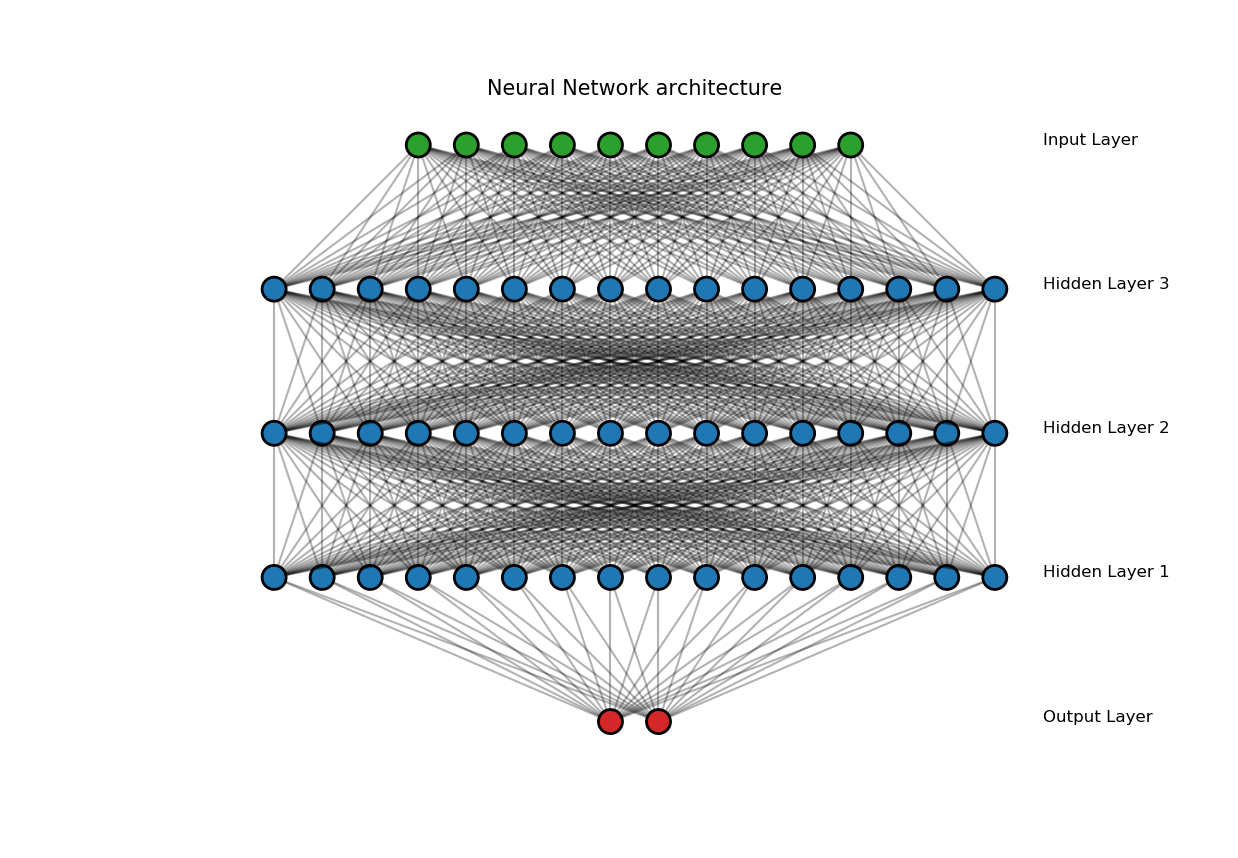
\includegraphics[width=\textwidth]{NN_NextStep_v2}
	\caption{Evaluation für die NextStep Prädiktion}
	% \todo{Quelle Bild!}
	\label{fig:boxplotErrorNNnextStep}
\end{figure}

- CV, CA
- Ergebnis Netz
- Ergebnis Lineare Regression


Vergleich Realdaten und simulierte Daten.
Realdaten mit ungefähr \SI{1.1}{\meter\per\second} während Simulierte mit \SI{1.5}{\metre\per\second} Bandgeschwindigkeit 

Zylinder schlechte performance erklären \textrightarrow orientierung fehlt

\section{Separator}

CV, CA quasi wie oben.
zusätzlich: CVBC, AA und IA

- Ergebnis NN
- Ergebnis Lineare Regression

\begin{figure}[h]
    \centering
    \missingfigure{Boxplots Result NeuralNets Separator}
	% 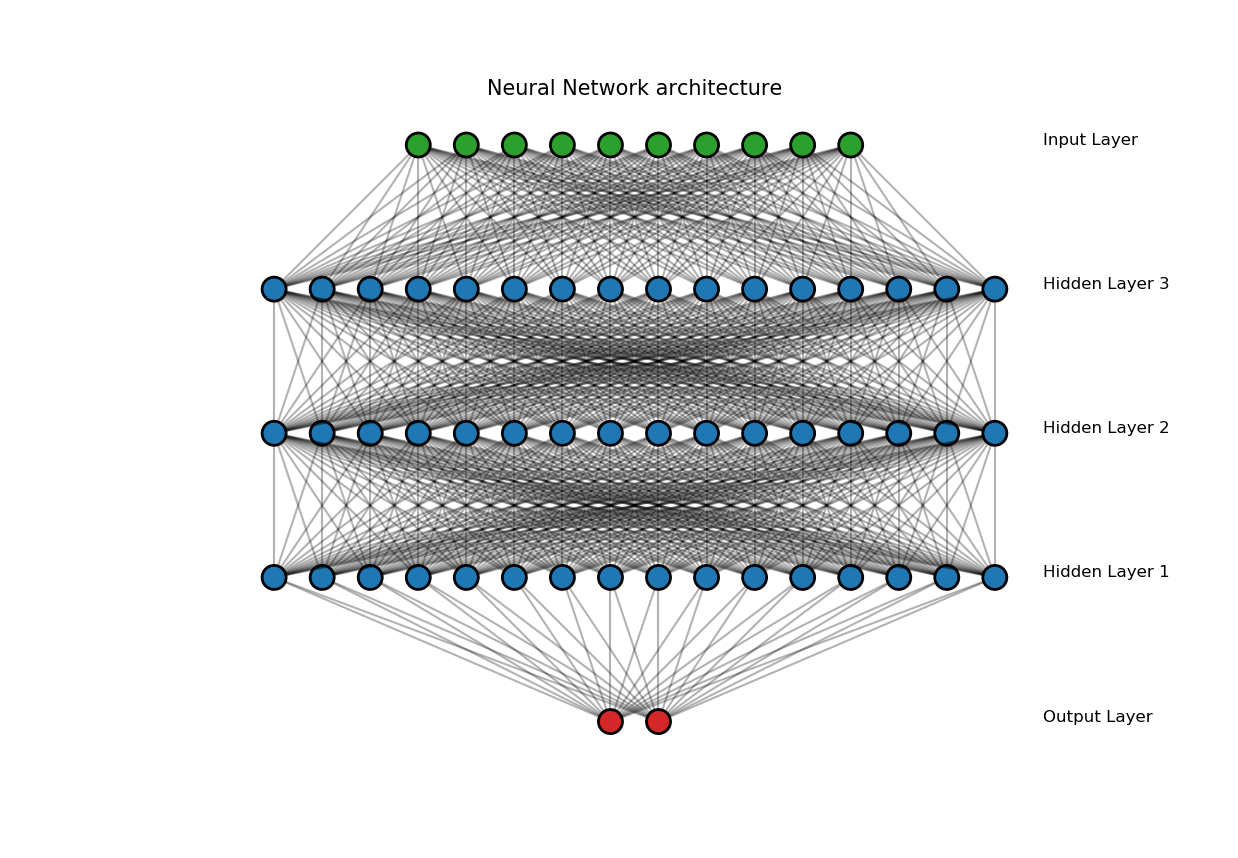
\includegraphics[width=\textwidth]{NN_NextStep_v2}
	\caption{Evaluation für die Separator Prädiktion}
	% \todo{Quelle Bild!}
	\label{fig:boxplotErrorNNSeparator}
\end{figure}